\begin{flushright} {\tiny {\color{gray} (tikz\_4x3x2.tex)}} \end{flushright}
%~~~~~~~~~~~~~~~~~~~~~~~~~~~~~~~~~~~~~~~~~~~~~~~~~~~~~~~~~~~~~~~~~~~~~~~~~~~~~~~~~~~~~~~~~~~~~~~~~~


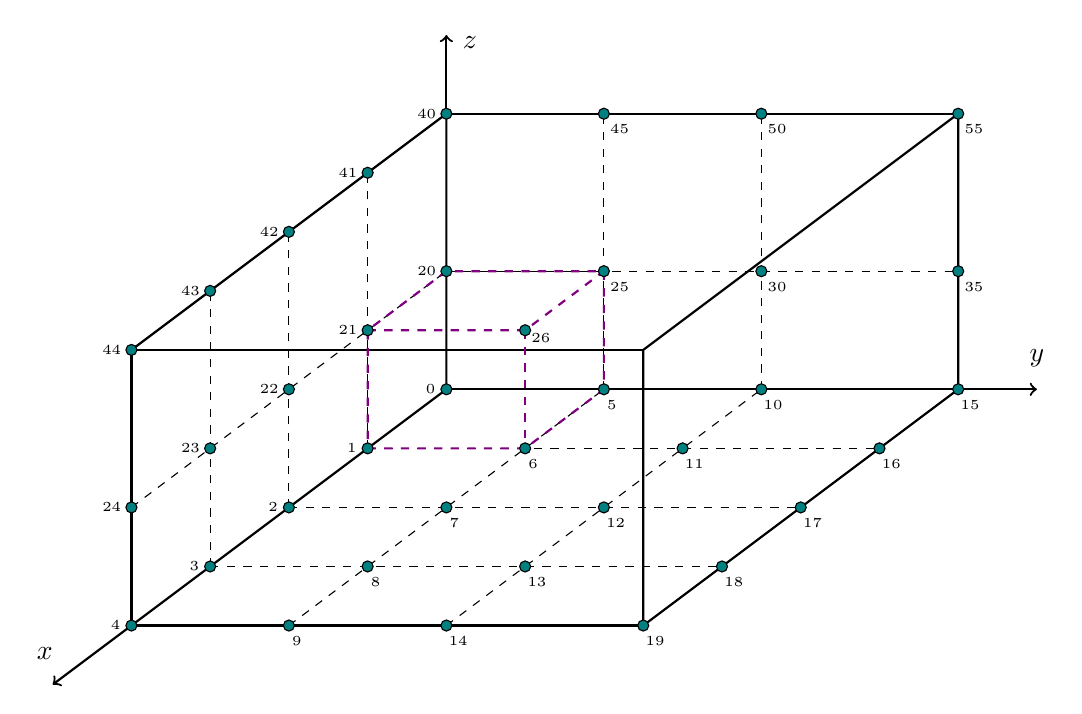
\begin{tikzpicture}
%\draw[step=0.5cm,gray,very thin] (0,0) grid (14,10); %background grid

%element
\draw[thick] (2,2) -- (8.5,2) -- (8.5,5.5) -- (2,5.5) -- cycle;  
\draw[thick] (2,2) -- (6,5) -- (6,8.5) -- (2,5.5) -- cycle ;
\draw[thick] (8.5,2) -- (12.5,5) -- (12.5,8.5) -- (8.5,5.5) -- cycle ;
\draw[thick] (6,5) -- (12.5,5) ;
\draw[thick] (6,8.5) -- (12.5,8.5) ;

%axes
\draw[thick,->] (2,2)--(1,1.25);
\draw[thick,->] (12.5,5)--(13.5,5);
\draw[thick,->] (6,8.5)--(6,9.5);
\node[] at (0.9,1.65) {$x$};
\node[] at (13.5,5.4) {$y$};
\node[] at (6.3,9.4) {$z$};

\draw[dashed] (2,3.5)--(6,6.5);
\draw[dashed] (3,2.75)--(3,6.25);
\draw[dashed] (4,3.5)--(4,7);
\draw[dashed] (5,4.25)--(5,7.75);
\draw[dashed] (4,2)--(8,5);
\draw[dashed] (6,2)--(10,5);
\draw[dashed] (3,2.75)--(9.5,2.75);
\draw[dashed] (4,3.5)--(10.5,3.5);
\draw[dashed] (5,4.25)--(11.5,4.25);
\draw[dashed] (6,6.5)--(12.5,6.5);
\draw[dashed] (8,5)--(8,8.5);
\draw[dashed] (10,5)--(10,8.5);

\draw[dashed, thick,violet] (5,4.25)--(7,4.25) --(8,5)--(8,6.5) --(6,6.5)--(5,5.75)--(5,4.25);
\draw[dashed, thick,violet] (5,5.75)--(7,5.75)--(8,6.5);
\draw[dashed, thick,violet] (7,5.75)--(7,4.25);

\draw[black,fill=teal] (2,2) circle (2pt); 
\draw[black,fill=teal] (3,2.75) circle (2pt); 
\draw[black,fill=teal] (4,3.5) circle (2pt); 
\draw[black,fill=teal] (5,4.25) circle (2pt); 
\draw[black,fill=teal] (6,5) circle (2pt); 

\draw[black,fill=teal] (2,3.5) circle (2pt); 
\draw[black,fill=teal] (3,4.25) circle (2pt); 
\draw[black,fill=teal] (4,5) circle (2pt); 
\draw[black,fill=teal] (5,5.75) circle (2pt); 
\draw[black,fill=teal] (6,6.5) circle (2pt); 

\draw[black,fill=teal] (2,5.5) circle (2pt); 
\draw[black,fill=teal] (3,6.25) circle (2pt); 
\draw[black,fill=teal] (4,7) circle (2pt); 
\draw[black,fill=teal] (5,7.75) circle (2pt); 
\draw[black,fill=teal] (6,8.5) circle (2pt); 

\draw[black,fill=teal] (4,2) circle (2pt); 
\draw[black,fill=teal] (5,2.75) circle (2pt); 
\draw[black,fill=teal] (6,3.5) circle (2pt); 
\draw[black,fill=teal] (7,4.25) circle (2pt); 
\draw[black,fill=teal] (8,5) circle (2pt); 

\draw[black,fill=teal] (6,2) circle (2pt); 
\draw[black,fill=teal] (7,2.75) circle (2pt); 
\draw[black,fill=teal] (8,3.5) circle (2pt); 
\draw[black,fill=teal] (9,4.25) circle (2pt); 
\draw[black,fill=teal] (10,5) circle (2pt); 

\draw[black,fill=teal] (8.5,2) circle (2pt); 
\draw[black,fill=teal] (9.5,2.75) circle (2pt); 
\draw[black,fill=teal] (10.5,3.5) circle (2pt); 
\draw[black,fill=teal] (11.5,4.25) circle (2pt); 
\draw[black,fill=teal] (12.5,5) circle (2pt);

\draw[black,fill=teal] (7,5.75) circle (2pt);


\draw[black,fill=teal] (8,6.5) circle (2pt);
\draw[black,fill=teal] (8,8.5) circle (2pt);

\draw[black,fill=teal] (10,6.5) circle (2pt);
\draw[black,fill=teal] (10,8.5) circle (2pt);

\draw[black,fill=teal] (12.5,6.5) circle (2pt);
\draw[black,fill=teal] (12.5,8.5) circle (2pt);

\node[] at (5.8,5) {\tiny 0};
\node[] at (4.8,4.25) {\tiny 1};
\node[] at (3.8,3.5) {\tiny 2};
\node[] at (2.8,2.75) {\tiny 3};
\node[] at (1.8,2) {\tiny 4};

\node[] at (5.75,6.5) {\tiny 20};
\node[] at (4.75,5.75) {\tiny 21};
\node[] at (3.75,5) {\tiny 22};
\node[] at (2.75,4.25) {\tiny 23};
\node[] at (1.75,3.5) {\tiny 24};

\node[] at (5.75,8.5) {\tiny 40};
\node[] at (4.75,7.75) {\tiny 41};
\node[] at (3.75,7) {\tiny 42};
\node[] at (2.75,6.25) {\tiny 43};
\node[] at (1.75,5.5) {\tiny 44};

\node[] at (8.1,4.8) {\tiny 5};
\node[] at (7.1,4.05) {\tiny 6};
\node[] at (6.1,3.3) {\tiny 7};
\node[] at (5.1,2.55) {\tiny 8};
\node[] at (4.1,1.8) {\tiny 9};

\node[] at (10.15,4.8) {\tiny 10};
\node[] at (9.15,4.05) {\tiny 11};
\node[] at (8.15,3.3) {\tiny 12};
\node[] at (7.15,2.55) {\tiny 13};
\node[] at (6.15,1.8) {\tiny 14};

\node[] at (12.65,4.8) {\tiny 15};
\node[] at (11.65,4.05) {\tiny 16};
\node[] at (10.65,3.3) {\tiny 17};
\node[] at (9.65,2.55) {\tiny 18};
\node[] at (8.65,1.8) {\tiny 19};

\node[] at (8.2,6.3) {\tiny 25};
\node[] at (7.2,5.65) {\tiny 26};

\node[] at (8.2,8.3) {\tiny 45};
\node[] at (10.2,6.3) {\tiny 30};
\node[] at (10.2,8.3) {\tiny 50};

\node[] at (12.7,6.3) {\tiny 35};
\node[] at (12.7,8.3) {\tiny 55};

\end{tikzpicture}
